\section{Theorie}
\label{sec:Theorie}
\begin{figure}
  \centering
  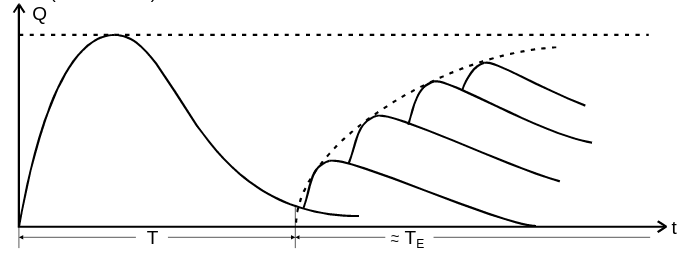
\includegraphics[width=\textwidth]{Bilder/erholzeit.png}
  \caption{Charakteristische Gestalt des Oszilloskopbild bei hohen Betriebsspannungen samt auftretender Nachentladungen. \cite{Anleitung}}
  \label{fig:nachladen}
\end{figure}


%Formel die ich brauchte:
\begin{equation}
  \label{eqn:totzeit}
  T \approx \frac{N_1+N_2-N_{1+2}}{2\cdot N_1N_2}
\end{equation}
